\begin{figure}[H]
\centering
\resizebox{\textwidth}{!}{%
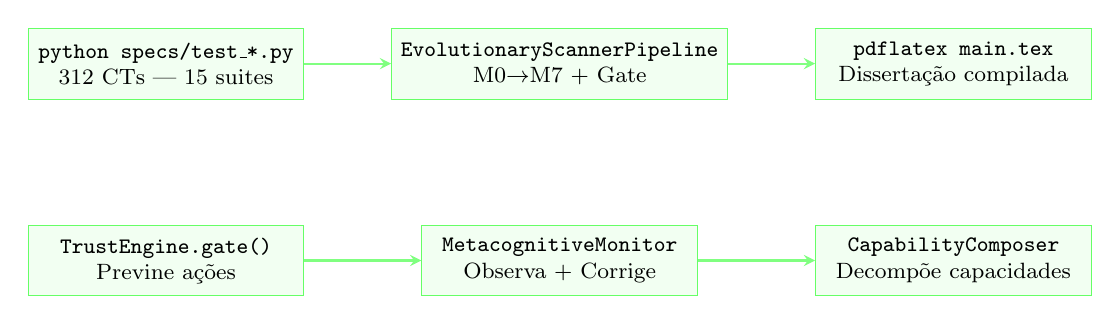
\begin{tikzpicture}[
    cmd/.style={rectangle, draw=green!60, fill=green!5, minimum width=3.5cm, minimum height=0.9cm, align=center, font=\footnotesize},
    arrow/.style={->, >=stealth, thick, green!50},
]
\node[cmd] (VERIFY) at (0,2) {\texttt{python specs/test\_*.py}\\312 CTs — 15 suites};
\node[cmd] (PIPELINE) at (5,2) {\texttt{EvolutionaryScannerPipeline}\\M0$\rightarrow$M7 + Gate};
\node[cmd] (COMPILE) at (10,2) {\texttt{pdflatex main.tex}\\Dissertação compilada};

\node[cmd] (GATE) at (0,-0.5) {\texttt{TrustEngine.gate()}\\Previne ações};
\node[cmd] (MONITOR) at (5,-0.5) {\texttt{MetacognitiveMonitor}\\Observa + Corrige};
\node[cmd] (COMPOSER) at (10,-0.5) {\texttt{CapabilityComposer}\\Decompõe capacidades};

\draw[arrow] (VERIFY) -- (PIPELINE);
\draw[arrow] (PIPELINE) -- (COMPILE);
\draw[arrow] (GATE) -- (MONITOR);
\draw[arrow] (MONITOR) -- (COMPOSER);
\end{tikzpicture}%
}
\caption{Comandos principais do OpenCode Ecosystem. Verificação: 312 CTs via \texttt{test\_*.py}. Pipeline: scanners M0$\rightarrow$M7 com Gate preventivo. Compilação: geração automatizada da dissertação. Ferramentas: BehavioralGate, MetacognitiveMonitor, CapabilityComposer.}
\label{fig:comandos}
\end{figure}
